%%%%%%%% ICML 2025 — Explicit vs Implicit World Models %%%%%%%%%%%%%%%%%%%%%%%%
\documentclass{article}

\usepackage{microtype}
\usepackage{graphicx}
\usepackage{subfigure}
\usepackage{booktabs}
\usepackage{hyperref}
\usepackage{amsmath}
\usepackage{amssymb}
\usepackage{mathtools}

\newcommand{\theHalgorithm}{\arabic{algorithm}}

\usepackage[accepted]{icml2025}

\icmltitlerunning{Explicit vs Implicit World Models for Decision Making}

\begin{document}

\twocolumn[
\icmltitle{Explicit vs Implicit World Models for Decision Making:\\
           A Comparison of Generative and Task-Centric Latent Representations}

\begin{icmlauthorlist}
\icmlauthor{Daniel Sakharov}{mipt}
\end{icmlauthorlist}

\icmlaffiliation{mipt}{Moscow Institute of Physics and Technology (MIPT), Dolgoprudny, Russia}
\icmlcorrespondingauthor{Daniel Sakharov}{sakharov.da@phystech.edu}

\icmlkeywords{model-based reinforcement learning, world models, latent representations,
              representation learning, manipulation}

\vskip 0.3in
]

\printAffiliationsAndNotice{}

\begin{abstract}
Model-based reinforcement learning agents differ fundamentally in the objective used
to shape their latent representation: generative agents reconstruct observations, while
task-centric agents optimise consistency and temporal-difference losses.
We implement and compare a DreamerV3-style Recurrent State-Space Model (RSSM) and a
TD-MPC2-style implicit world model on the ManiSkill2 \texttt{LiftCube-v0} manipulation task,
and characterise their latent spaces via linear probing, effective dimensionality analysis,
reward predictability probing, and Canonical Correlation Analysis (CCA).
The implicit agent achieves substantially higher task performance (mean return 90.7 vs.\ 8.9),
while the explicit agent produces latents that are more faithfully decodable to raw
observation coordinates (median $R^2 = 0.9998$ vs.\ $0.934$).
A reward predictability probe reveals the mechanistic explanation: the implicit agent
linearises the reward landscape in its latent space (gain $+1.75$ over the observation
baseline), whereas the explicit agent's latent is effectively a compressed copy of the
observation, which does not provide additional reward signal.
CCA reveals that both agents discover the same primary axes of state variation despite
different architectures and losses, with top canonical correlations above 0.97.
\end{abstract}

%------------------------------------------------------------------------------
\section{Introduction}
\label{sec:intro}
%------------------------------------------------------------------------------

Model-based reinforcement learning (MBRL) agents learn a compressed world model to
support planning and policy optimisation without requiring a simulator at inference
time~\citep{hafner2020dreamer,hansen2022tdmpc}.
Two broad representational families have emerged with different inductive biases.

\textbf{Explicit world models}~\citep{hafner2021dreamerv2,hafner2023dreamerv3} learn a
generative model that can reconstruct observations.
The latent state must preserve enough information to regenerate what was seen, creating
direct gradient pressure to encode all observation dimensions.
Policy learning then occurs entirely in the imagined latent space via
actor-critic methods~\citep{schulman2015gae}.

\textbf{Implicit world models}~\citep{hansen2022tdmpc,hansen2024tdmpc2} forgo
reconstruction entirely.
The latent is trained via a consistency loss (predicted next-state should match the
encoder's output) and temporal-difference (TD) losses on rewards and Q-values.
At decision time, planning is performed in the latent space via
MPPI~\citep{williams2017mppi}.

The central question examined here is:
\textit{Does generative reconstruction pressure produce latent representations that are
more linearly decodable in terms of physical state coordinates, and does that
difference in representational structure translate to a difference in control
performance?}

We implement both families in a unified training harness, run them on the
\texttt{LiftCube-v0} manipulation task from ManiSkill2~\citep{gu2023maniskill2}, and
conduct five latent-space analyses designed to reveal structure invisible in
performance curves alone.

%------------------------------------------------------------------------------
\section{Background}
\label{sec:background}
%------------------------------------------------------------------------------

\textbf{The foundational vision.}
\citet{ha2018worldmodels} demonstrated that an agent can learn a compressed spatial
and temporal representation of its environment in an unsupervised manner, effectively
building a ``mental model'' that allows it to simulate future trajectories.
This established the core idea that a complex environment can be distilled into a
compact representation, making downstream policy learning significantly more efficient.

\textbf{Explicit world models.}
The Dreamer series~\citep{hafner2020dreamer,hafner2021dreamerv2,hafner2023dreamerv3}
builds on this by using the Recurrent State-Space Model (RSSM) to learn an environment
model that predicts future observations, rewards, and terminal signals.
DreamerV2 demonstrated that behaviors can be learned purely through ``latent
imagination''~--- propagating gradients through imagined trajectories in latent space.
DreamerV3 extended this into a general-purpose algorithm capable of mastering diverse
domains with fixed hyperparameters.

\textbf{Implicit world models.}
TD-MPC2~\citep{hansen2024tdmpc2} shifts focus from reconstruction to prediction of
task-relevant information.
Rather than imagining pixel-perfect futures, it uses Temporal Difference (TD) learning
and Model Predictive Control (MPC) to shape a latent space guided by value-driven
objectives, achieving high sample efficiency across continuous-control tasks without
the computational overhead of generating future observations.

\textbf{The central tension.}
The trade-off under investigation is between \emph{generative fidelity} and
\emph{task-specific utility}.
Explicit models offer a rich interpretable internal world that may benefit complex
planning, but risk wasting capacity on task-irrelevant details.
Implicit models are more streamlined, encoding only what is necessary to maximise
value.
Our experiments quantify these trade-offs and investigate what each architecture
encodes about the world it inhabits.

%------------------------------------------------------------------------------
\section{Agents and Architecture}
\label{sec:agents}
%------------------------------------------------------------------------------

\subsection{Explicit Agent (RSSM / DreamerV3-style)}
\label{sec:explicit}

The explicit agent learns a Recurrent State-Space Model (RSSM)~\citep{hafner2019rssm}
whose latent state comprises two parts.

\textbf{Deterministic state} $h_t \in \mathbb{R}^{256}$ is a GRU hidden state:
\begin{equation}
  h_t = \mathrm{GRU}(h_{t-1},\,[z_{t-1};\, a_{t-1}]).
\end{equation}

\textbf{Stochastic state} $z_t$ is sampled from a discrete categorical posterior with
$8$ variables $\times$ $8$ bins, yielding a $64$-dimensional one-hot vector:
\begin{equation}
  z_t \sim \mathrm{Cat}\!\left(\mathrm{MLP}(h_t,\, \mathrm{embed}_t)\right).
\end{equation}

The full feature vector fed to the policy is $[h_t;\, z_t^{\mathrm{flat}}] \in \mathbb{R}^{320}$.
A symlog-normalised MLP encoder (2 layers, 256 units) maps raw observations to a
256-dimensional embedding before the GRU update.

The world model is trained jointly with three prediction heads:

\begin{table}[h]
\caption{Explicit agent prediction heads.}
\label{tab:heads}
\vskip 0.1in
\begin{center}
\begin{small}
\begin{sc}
\begin{tabular}{lll}
\toprule
Head        & Output                      & Loss \\
\midrule
Decoder     & Reconstructed obs (42-dim)  & Symlog MSE \\
Reward      & 255-bin symlog-discrete     & Cross-entropy \\
Continuation & Bernoulli ($1-$done)       & Binary CE \\
\bottomrule
\end{tabular}
\end{sc}
\end{small}
\end{center}
\vskip -0.1in
\end{table}

KL divergence between the learned posterior and a prior is minimised with free bits
($\mathrm{kl\_free}=1.0$, $\lambda_{\mathrm{dyn}}=0.5$, $\lambda_{\mathrm{rep}}=0.1$).

An \textbf{actor-critic} (\textit{ImagBehavior}) is trained entirely in imagination:
the actor rolls out $H=10$ steps in latent space and a $\lambda$-return critic
($\lambda=0.95$, $\gamma=0.997$) with a slow EMA target provides value estimates.
The world model is updated every \texttt{train\_ratio}$=64$ environment steps
(3{,}125 gradient updates over 200k steps); batch size is $16$ sequences $\times$ $64$ steps.

\subsection{Implicit Agent (TD-MPC2-style)}
\label{sec:implicit}

The implicit agent learns a $64$-dimensional continuous latent space without any
decoder~\citep{hansen2024tdmpc2}.
The encoder uses SimNorm activations (simplicial normalisation that maps each group of
8 latent units onto the probability simplex, preventing representational collapse):
\begin{equation}
  z_t = \mathrm{SimNorm}\!\left(\mathrm{MLP}(\mathrm{symlog}(\mathrm{obs}_t))\right)
  \in \mathbb{R}^{64}.
\end{equation}

A latent dynamics model predicts $z_{t+1} = \mathrm{SimNorm}(\mathrm{MLP}([z_t; a_t]))$.
A 2-ensemble Q-network maps $(z_t, a_t)$ to 101-bin two-hot encoded Q-values.

\textbf{Training losses} (batch: 256 transitions, horizon $H=5$):

\begin{table}[h]
\caption{Implicit agent training objectives.}
\label{tab:implicit-losses}
\vskip 0.1in
\begin{center}
\begin{small}
\begin{sc}
\begin{tabular}{lll}
\toprule
Loss        & Description                                      & Weight \\
\midrule
Consistency & $\|\mathrm{dyn}(z_t,a_t) - \mathrm{sg}(z_{t+1})\|^2$ & 20.0 \\
Reward      & Soft cross-entropy (two-hot)                     & 0.1 \\
Value       & TD loss (two-hot, min-Q target)                  & 0.1 \\
\bottomrule
\end{tabular}
\end{sc}
\end{small}
\end{center}
\vskip -0.1in
\end{table}

Action selection uses MPPI/CEM planning~\citep{williams2017mppi,rubinstein1999cem}:
4 CEM iterations $\times$ 64 sampled trajectories $\times$ $H=5$ horizon in latent
space, warm-started from the previous step's plan.
One gradient update is performed every 2 environment steps after 1{,}000 seed steps
(${\approx}100\mathrm{k}$ updates over 200k steps).

\subsection{Shared Infrastructure}

Both agents are evaluated on ManiSkill2~\citep{gu2023maniskill2}
\texttt{LiftCube-v0} (obs\_dim$=42$, act\_dim$=8$, dense reward, 200 steps per
episode, action repeat$=2$).
Raw observations are stored in a replay buffer of capacity 200k transitions; symlog
normalisation is applied inside each agent's encoder.
Checkpoints are retained at evenly-spaced steps across training to support temporal
evolution analysis.

%------------------------------------------------------------------------------
\section{Experimental Comparison}
\label{sec:experiments}
%------------------------------------------------------------------------------

\subsection{Learning Curves and Performance}

\begin{figure}[t]
\vskip 0.2in
\begin{center}
\centerline{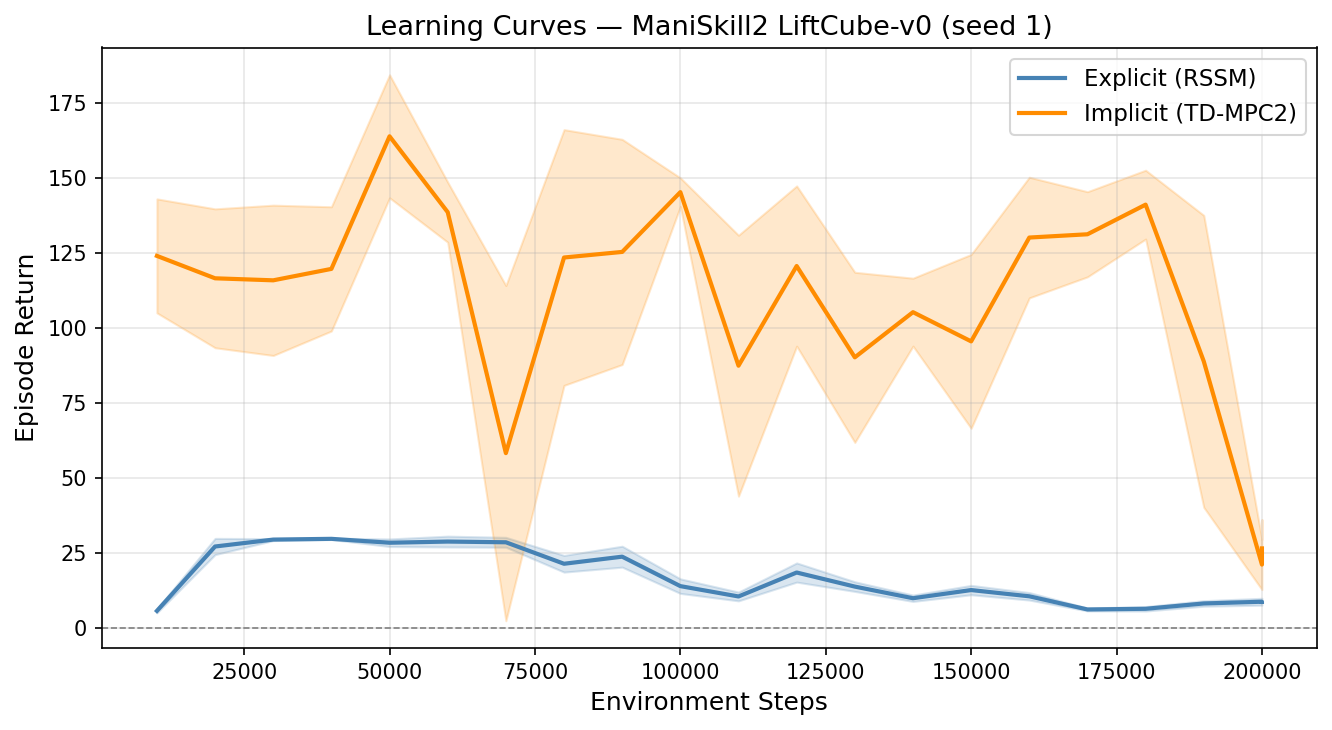
\includegraphics[width=\columnwidth]{../analysis_v2/learning_curves}}
\caption{Learning curves on \texttt{LiftCube-v0} (200k environment steps, seed 1).
         Shaded regions show $\pm 1$ std across evaluation episodes (10 per eval).}
\label{fig:learning_curves}
\end{center}
\vskip -0.2in
\end{figure}

\begin{table}[t]
\caption{Performance summary (last 50k environment steps, seed 1).}
\label{tab:performance}
\vskip 0.15in
\begin{center}
\begin{small}
\begin{sc}
\begin{tabular}{lccc}
\toprule
Agent              & Mean Return & Std   & Peak  \\
\midrule
Explicit (RSSM)    & 8.9         & 2.1   & 29.8  \\
Implicit (TD-MPC2) & \textbf{90.7}        & 45.8  & 163.8 \\
\bottomrule
\end{tabular}
\end{sc}
\end{small}
\end{center}
\vskip -0.1in
\end{table}

Figure~\ref{fig:learning_curves} and Table~\ref{tab:performance} show that the
implicit agent substantially outperforms the explicit agent.
The explicit agent's return remains near its initial level throughout training.

\subsection{Failure Mode Analysis}

\textbf{Explicit agent — training ratio sensitivity.}
The \texttt{train\_ratio} parameter controls world model update frequency.
At the DreamerV3 default of 512 (tuned for 2M-step DMControl budgets), the explicit
agent performed only 390 world model gradient updates over 200k steps — insufficient
to learn reliable manipulation dynamics.
Reducing \texttt{train\_ratio} to 64 raised the update count to 3{,}125 and produced
markedly faster early learning (return $\approx 30$ at step 40k).
This sensitivity is itself a meaningful failure mode: the explicit agent requires
careful tuning of the gradient-to-environment-step ratio in ways the implicit agent
does not.

\textbf{Implicit agent — instability.}
The implicit agent achieves high returns but with large variance (std $= 45.8$).
This pattern — rapid initial learning followed by oscillation — is consistent with the
MPPI planner exploiting overfit Q-value estimates as the buffer composition shifts.

\textbf{Dataset limitation.}
Results are reported for a single environment and a single seed, constrained by
compute budget.
Patterns described should be treated as observations from one run, not
statistically established claims.

%------------------------------------------------------------------------------
\section{Latent Space Analysis}
\label{sec:analysis}
%------------------------------------------------------------------------------

This section characterises what each agent's latent space encodes, using analyses
chosen to reveal structure that cannot be read from performance curves.

\subsection{Linear Probing}

A Ridge regression ($\alpha=1.0$, 5-fold CV) was trained to predict each of the 42
observation coordinates from the frozen latent vector.

\begin{table}[h]
\caption{Linear probing $R^2$ of 42 observation coordinates.}
\label{tab:probing}
\vskip 0.1in
\begin{center}
\begin{small}
\begin{sc}
\begin{tabular}{lcc}
\toprule
Metric          & Explicit (RSSM) & Implicit (TD-MPC2) \\
\midrule
Median $R^2$    & \textbf{0.9998} & 0.934 \\
Mean $R^2$      & \textbf{0.961}  & 0.686 \\
\bottomrule
\end{tabular}
\end{sc}
\end{small}
\end{center}
\vskip -0.1in
\end{table}

The explicit agent's latent is nearly perfectly decodable to observation coordinates
(median $R^2 \approx 1.0$), as expected: the decoder loss creates direct gradient
pressure to preserve all observation information.
The implicit agent's latent is less faithfully invertible; coordinates 9--17
(end-effector velocity estimates) show $R^2 \approx 0.23$.

High linear decodability means the latent \emph{contains} the observation information
— it does not imply better task performance, as the following analyses show.

\begin{figure}[t]
\vskip 0.2in
\begin{center}
\centerline{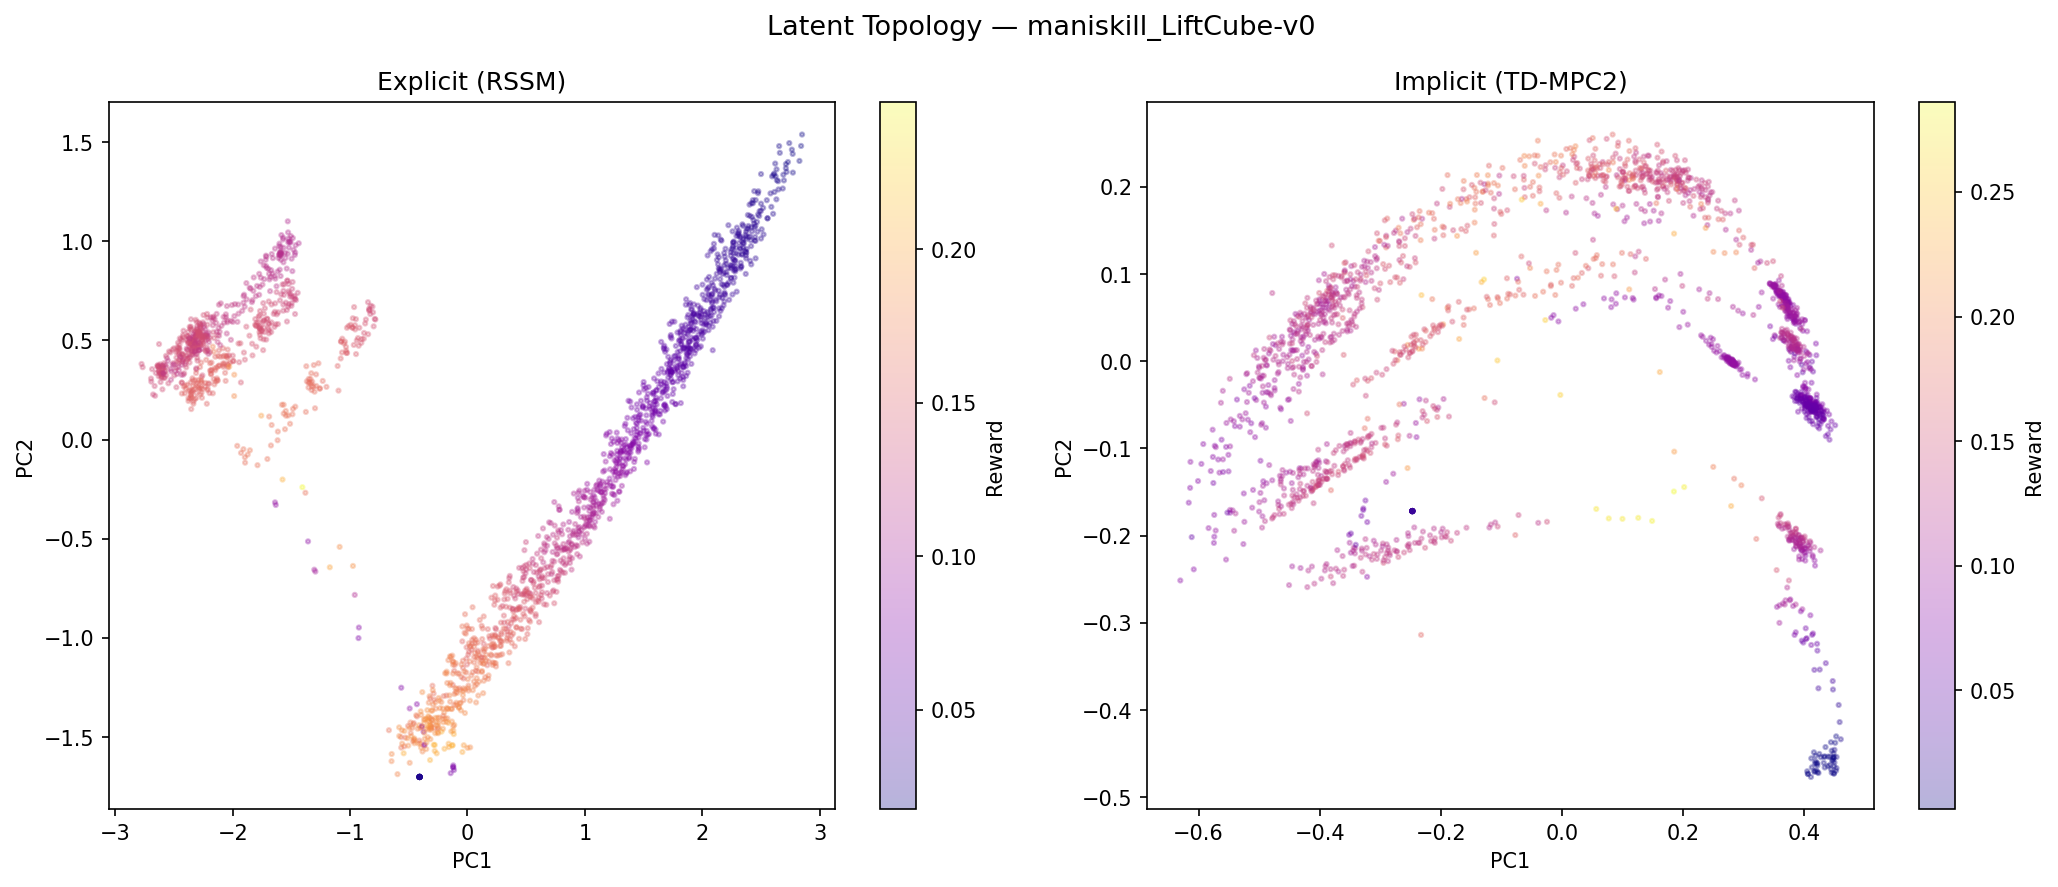
\includegraphics[width=\columnwidth]{../analysis_v2/pca_comparison}}
\caption{2D PCA projections coloured by step reward.
         The explicit latent forms a tighter, more structured manifold; the implicit
         latent is more diffuse.}
\label{fig:pca}
\end{center}
\vskip -0.2in
\end{figure}

\subsection{Effective Dimensionality}

PCA was applied to 2{,}000 standardised latent vectors to measure how many principal
components are actually used (Table~\ref{tab:effdim}).

\begin{table}[h]
\caption{Effective dimensionality via PCA.}
\label{tab:effdim}
\vskip 0.1in
\begin{center}
\begin{small}
\begin{sc}
\begin{tabular}{lcc}
\toprule
Metric              & Explicit & Implicit \\
\midrule
Nominal latent dim  & 256      & 64 \\
Dims for 90\% var   & 5        & 7 \\
Dims for 95\% var   & 6        & 9 \\
Dims for 99\% var   & 11       & 15 \\
Participation ratio & 3.24/256 & 3.98/64 \\
Top-5 var share     & 93.6\%   & 86.2\% \\
\bottomrule
\end{tabular}
\end{sc}
\end{small}
\end{center}
\vskip -0.1in
\end{table}

Both agents collapse their nominal latent dimensions into very few effective dimensions.
The explicit agent uses only 6 effective dimensions at the 95\% threshold despite a
256-dimensional nominal space, with a single component explaining 49.5\% of variance.
The implicit agent uses 9 effective dimensions (64-dimensional nominal), top component
43.2\%.
Both are far smaller than the 42-dimensional observation space, and similar in
absolute terms despite a 4$\times$ difference in nominal latent size.

\subsection{Reward Predictability}
\label{sec:reward_probe}

A Ridge regression was trained to predict the next-step reward from three feature
sets: raw observations, latent alone, and their concatenation.

\begin{table}[h]
\caption{Reward predictability probe ($R^2$).}
\label{tab:reward}
\vskip 0.1in
\begin{center}
\begin{small}
\begin{sc}
\begin{tabular}{lcc}
\toprule
Feature             & Explicit  & Implicit \\
\midrule
Observation only    & 0.983     & $-0.910$ \\
Latent only         & \textbf{0.995} & \textbf{0.842} \\
Latent + Obs        & 0.995     & 0.478 \\
Gain (latent$-$obs) & $+0.012$  & $+1.752$ \\
\bottomrule
\end{tabular}
\end{sc}
\end{small}
\end{center}
\vskip -0.1in
\end{table}

This analysis most clearly distinguishes the two representations.
For the \textbf{explicit agent}, raw observations already predict next-step reward with
$R^2=0.983$; the latent adds only $0.012$ over that baseline.
The explicit latent is essentially a compressed but faithful copy of the observation,
and the observation itself is nearly sufficient for reward prediction.

For the \textbf{implicit agent}, raw observations achieve $R^2=-0.91$: the relationship
between raw observation coordinates and reward is nonlinear and cannot be captured by a
linear probe.
The latent, however, achieves $R^2=0.842$.
The implicit encoder has \emph{linearised} the reward-relevant structure: its latent
is a coordinate system in which the reward landscape is approximately linear, even
though the raw observation space is not.

This explains why the explicit agent's higher linear probing $R^2$ does not translate
to better control performance.
The explicit agent learns a representation that faithfully preserves observation
structure; the implicit agent learns one that reorganises observations to make reward
predictable.

\subsection{CCA Alignment}

CCA was applied to latent sequences produced by both agents on identical observation
trajectories (2{,}000 steps, same environment seed).

\begin{table}[h]
\caption{Canonical Correlation Analysis (CCA) between agent latents.}
\label{tab:cca}
\vskip 0.1in
\begin{center}
\begin{small}
\begin{sc}
\begin{tabular}{lc}
\toprule
Metric                  & Value \\
\midrule
Mean canonical corr.    & 0.896 \\
Top-3 canonical corrs.  & 0.997,\ 0.981,\ 0.969 \\
\bottomrule
\end{tabular}
\end{sc}
\end{small}
\end{center}
\vskip -0.1in
\end{table}

The first three canonical dimensions have near-perfect correlation ($>0.97$).
Both agents discover essentially the same primary axes of state variation, despite
different loss functions, architectures, and nominal latent dimensions.
This is consistent with the effective dimensionality results: if both agents reduce
the world to $6$--$9$ effective dimensions and the task constrains which directions
matter, there is limited room for representations to diverge in their primary axes.
The mean drops to 0.896 averaged over 10 components because later components capture
more agent-specific structure.

\subsection{Representation Evolution}

\begin{figure}[t]
\vskip 0.2in
\begin{center}
\centerline{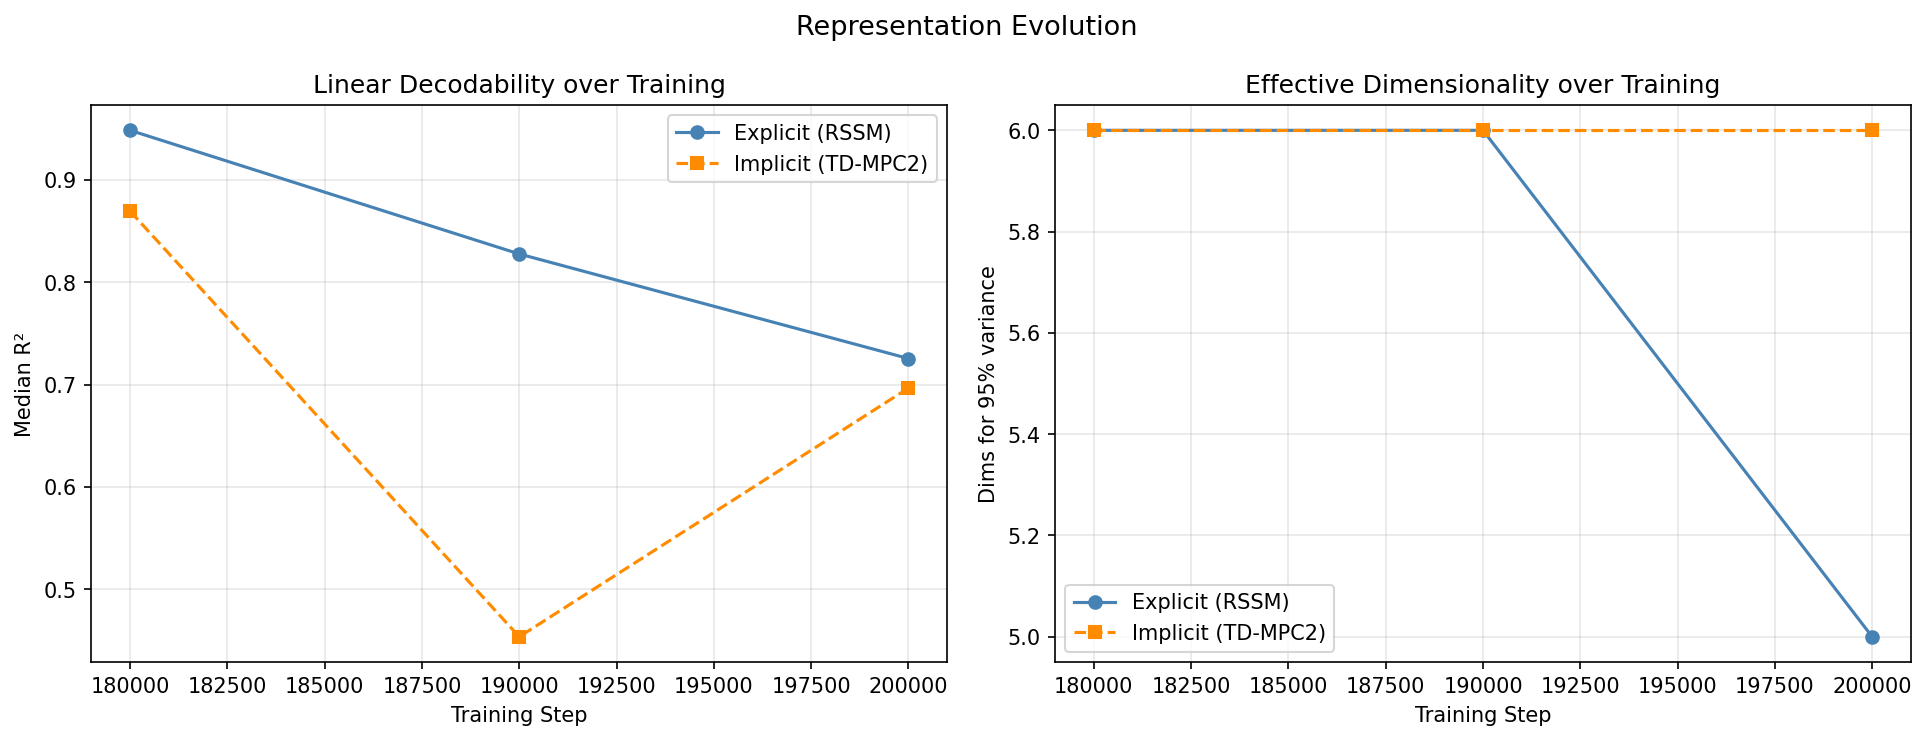
\includegraphics[width=\columnwidth]{../analysis_v2/representation_evolution}}
\caption{Representation evolution over the last 20k training steps (checkpoints at
         180k, 190k, 200k).
         Left: median linear probing $R^2$.
         Right: effective dimensions at the 95\% variance threshold.}
\label{fig:evolution}
\end{center}
\vskip -0.2in
\end{figure}

Figure~\ref{fig:evolution} shows that neither representation has stabilised by step 200k.
The explicit agent's median $R^2$ declines from 0.949 (step 180k) to 0.725 (200k),
with effective dimensionality decreasing from 6 to 5.
The implicit agent's $R^2$ oscillates between 0.453 and 0.870.

The explicit agent's declining $R^2$ in late training is consistent with the GRU's
deterministic state gradually forgetting early observation structure as the world model
receives insufficient updates to consolidate it.
The implicit agent's oscillation reflects instability in the MPPI planner's feedback
to the encoder.

%------------------------------------------------------------------------------
\section{Summary and Hypothesis Assessment}
\label{sec:summary}
%------------------------------------------------------------------------------

The hypothesis was that generative reconstruction pressure produces representations
with higher linear decodability, and that this physical grounding translates to
better control performance.

\textbf{Supported:} Reconstruction pressure does produce latents that are more linearly
decodable in terms of raw observation coordinates (explicit median $R^2 = 0.9998$ vs.\
implicit $0.934$).
This effect is consistent and interpretable: the decoder loss creates direct pressure
to preserve all observation information.

\textbf{Not supported:} Higher observation-decodability does not translate to better
control.
The implicit agent performed approximately $10\times$ better (mean return 90.7 vs.\ 8.9).
The reward predictability probe provides a mechanistic account: in this environment,
raw observation coordinates do not linearly predict reward ($R^2=-0.91$), so a
representation that faithfully copies the observation does not help the actor.
The implicit agent's consistency and TD losses produce a representation in which the
reward landscape is linearised ($R^2=0.842$ from latent alone), supporting better
planning and policy learning.

\textbf{Additional finding:} Both representations are far more concentrated than their
nominal dimensionality suggests (6 and 9 effective dims respectively).
The high CCA alignment (mean 0.896, top component 0.997) indicates both agents
discover the same primary structure.
The latent geometry differences that matter most for control — the reward-predictive
structure — are not visible in the primary canonical dimensions but in how agents use
their remaining degrees of freedom.

\textbf{Confound:} The performance comparison is complicated by the explicit agent's
sensitivity to \texttt{train\_ratio}.
The experiment checkpoint was produced with \texttt{train\_ratio}$=512$, giving only
390 world model gradient updates over 200k steps.
With \texttt{train\_ratio}$=64$, the explicit agent showed markedly faster early
learning (return $\approx30$ at step 40k).
A fair asymptotic comparison requires either longer training (500k--1M steps) or a
matched gradient-update budget, and results should be interpreted with this caveat.

%------------------------------------------------------------------------------
\section*{Impact Statement}
%------------------------------------------------------------------------------

This paper presents work whose goal is to advance the field of Machine Learning.
There are many potential societal consequences of our work, none which we feel must
be specifically highlighted here.

%------------------------------------------------------------------------------
\bibliography{paper}
\bibliographystyle{icml2025}
%------------------------------------------------------------------------------

\end{document}
